\chapter{Object Definitions}

% **************************** Define Graphics Path **************************
\ifpdf
    \graphicspath{{Chapter4/Figs/Raster/}{Chapter4/Figs/PDF/}{Chapter4/Figs/}}
\else
    \graphicspath{{Chapter4/Figs/Vector/}{Chapter4/Figs/}}
\fi


%********************************** % First Section  *************************************
\section{Introduction}  %Section - 1.1 
\label{sec:objects_introduction}

Physics objects are observed as energy deposits in the various detector 
subsystems throughout the CMS detector. Specific definitions for the different 
objects are provided by the Physics Object Groups (\emph{POGs}) and are used in this 
analysis. The following sections describe the objects used.


%********************************** % Second Section  *************************************
\section{Jets}  %Section - 1.2
\label{sec:objects_jets}

Jets are produced when a single quark or gluon is produced, subsequently 
hadronizing and showering throughout the calorimeter systems. Energy deposits in
the hadronic calorimeter are clustered using the anti-$k_T$ algorithm \cite{antikt} with
a $R=0.5$ cone size parameter. The raw energy measurements are subject to 
effects from overlapping pp collisions (PU), therefore corrections are made to
account for this \cite{Cacciari2008119, 1126-6708-2008-04-005}. Clustered jets 
are also corrected to establish a uniform response in $\eta$ and \Pt
\cite{Chatrchyan:2011ds}.
Table~\ref{tab:jet_id_loose} summarises the ID requirements used in this 
analysis, which correspond to the ``Loose'' working point \cite{ref:jet-id} 
(private!). Jets are further 
corrected according to the L1FastJet, L2, L3, and L2L3Residual corrections
\cite{ref:jet-jes} (private!).

\begin{table}[!ht]
  \caption{Criteria for the ``loose'' jet ID working point.\label{tab:jet_id_loose}}
  \footnotesize
  \begin{center}
    \begin{tabular}{ll}
      \hline
      \hline
      Requirement                & Description                                                      \\
      \hline
      f$_{HPD} < 0.98$           & Fractional contribution from the ``hottest'' Hybrid Photo Diode. \\
      f$_{EM} > 0.01$            & Minimum electromagnetic fractional component.                    \\
      N$^{90}_{\rm hits} \geq$ 2 & Number of HCAL channels containing at least
      90\% of total energy      \\
      \hline
      \hline
    \end{tabular}
  \end{center}
\end{table}


\subsection{Tagging jets from b-quarks}

Jets originating from b-quarks can be identified using information from the 
vertex detector due to their increased lifetime with respect to light
flavour quarks (u, d, s) and charm quarks. 
B-tagging algorithms are designed to determine the probability that a jet 
originates from a b-quark, given, amongst other properties, track
displacement from the primary vertex (PV). Each algorithm
calculates a value used to discriminate between a jet originating from a
b-quark and a light or c-quark.

\begin{figure}[h!]
  \centering
  \begin{subfigure}[b]{0.46\textwidth}
    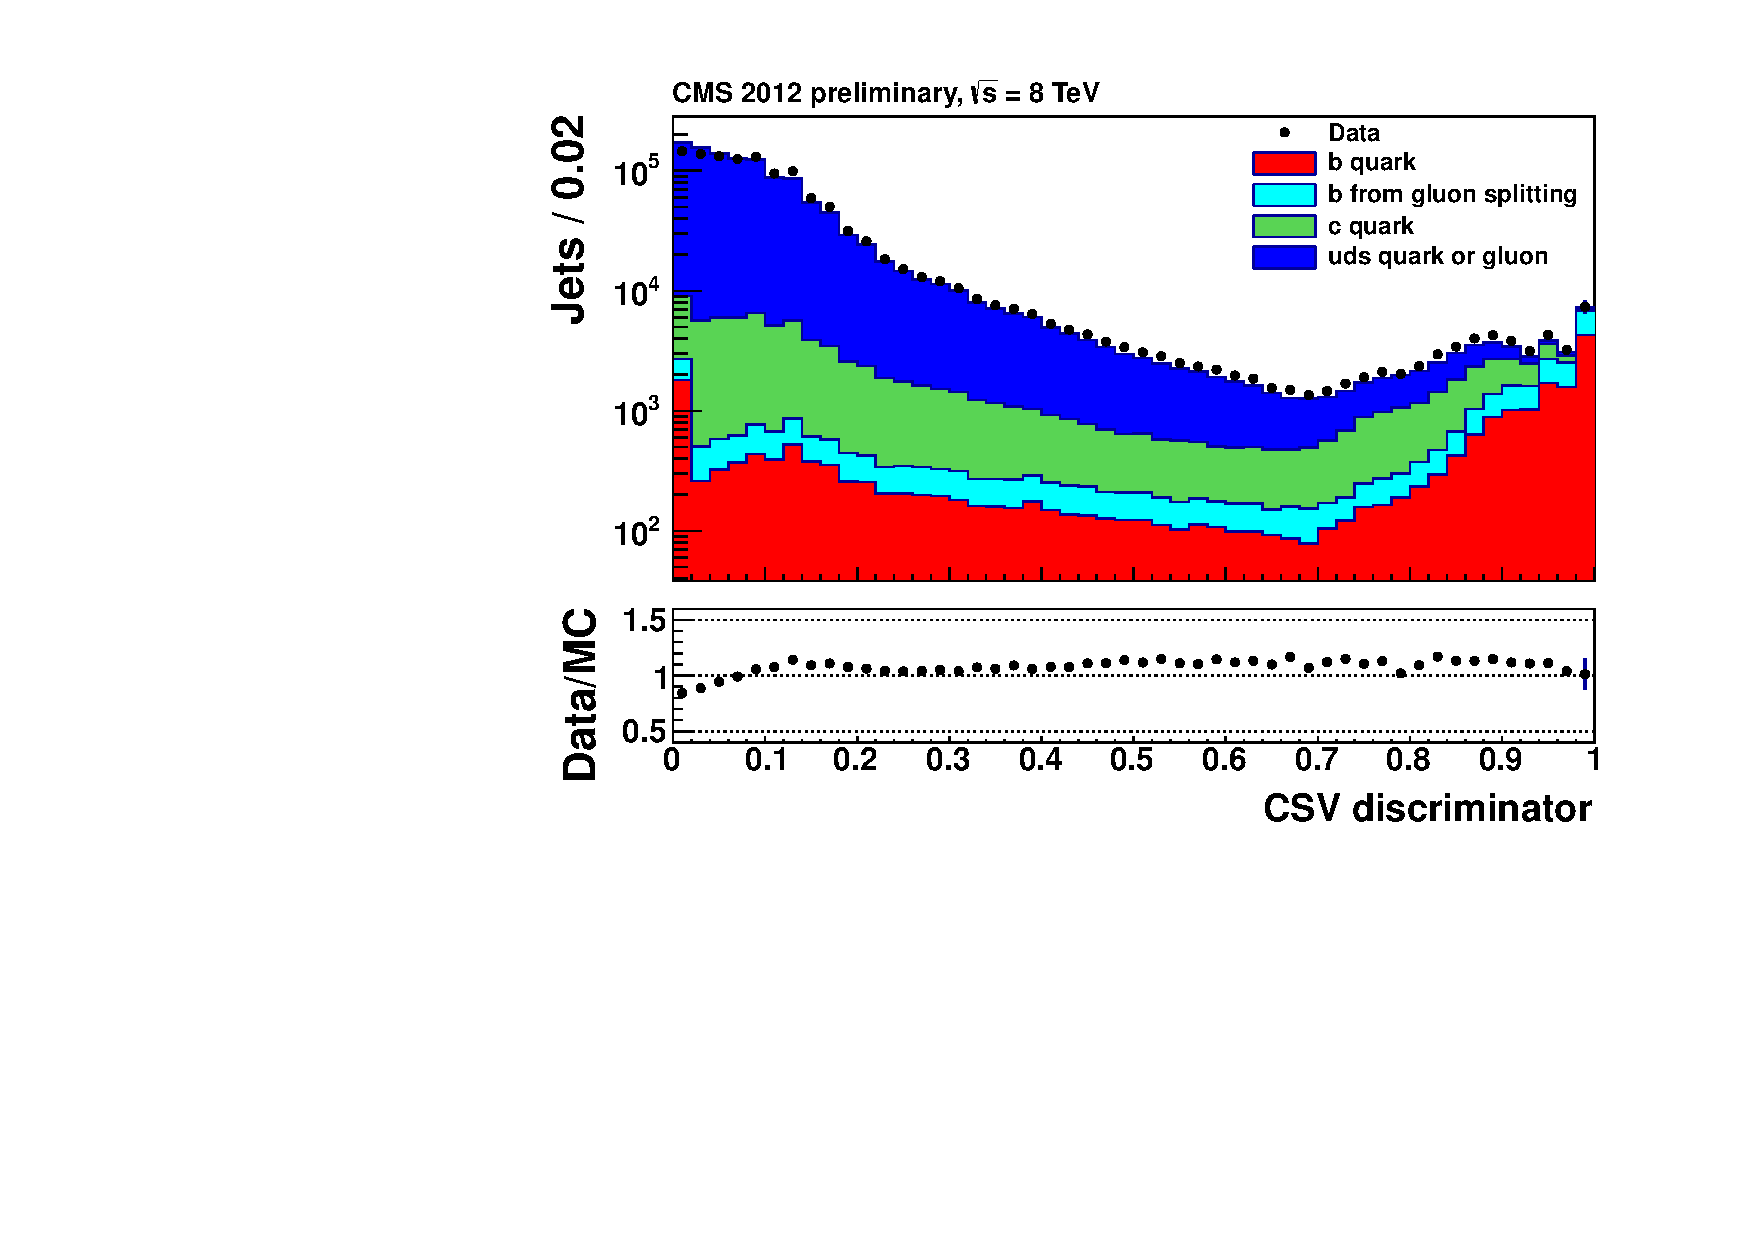
\includegraphics[width=\textwidth]{Figs/btag/csv_discrim.pdf}
    \caption{CSV Discriminator}
    \label{fig:btag_csv_discrim}
  \end{subfigure}
  \begin{subfigure}[b]{0.46\textwidth}
    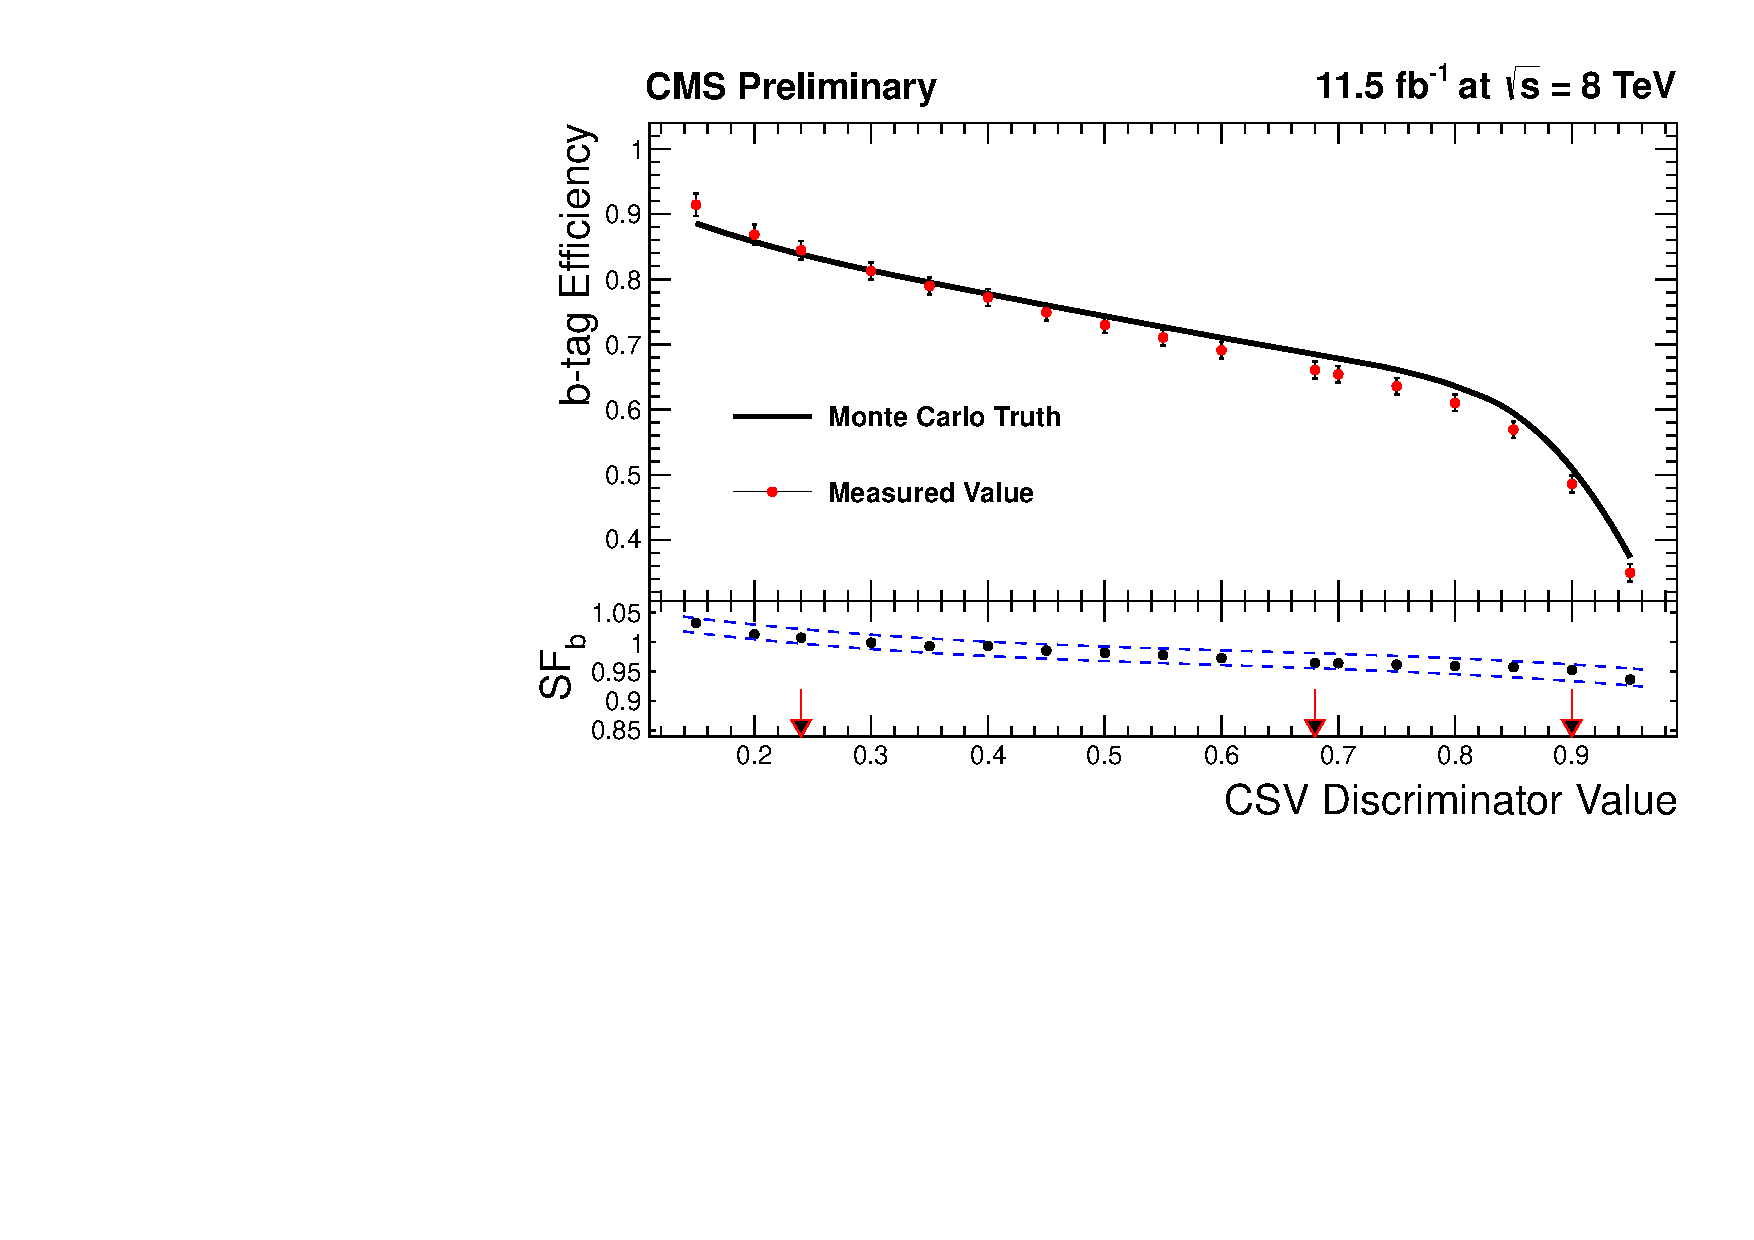
\includegraphics[width=\textwidth]{Figs/btag/csv_eff.pdf}
    \caption{CSV Efficiency}
    \label{fig:btag_csv_eff}
  \end{subfigure}
  \caption{The Combined Secondary Vertex b-tagging algorithm disciminator
  distribution (left) and the b-tagging efficiency (right) as measured in both
  data and simulation. MC scale factors are shown in the lower plot of
  \ref{fig:btag_csv_eff}.}
  \label{fig:btag_csv}
\end{figure}

The Combined Secondary Vertex (CSV) algorithm \cite{CMS-PAS-BTV-12-001} is used
in this analysis. The tagging algorithm calculates a discriminator value for
each jet, the distribution being shown in figure~\ref{fig:btag_csv_discrim}.
The ``Medium'' working point, or a discriminator
threshold of $>0.679$, is used in this analysis. This working point corresponds
to a mistag rate for gluons/light-quarks of 1\%, and a pT dependent efficiency
in the range of 60-70\%, as shown in figure~\ref{fig:btag_csv_eff}. Also
shown in figure~\ref{fig:btag_csv_eff} are the MC scale factors, $SF_b$, defined
as the ratio of the CSV b-tagging algorithm efficiency in data and MC, to be
applied to MC samples.


%********************************** % Fourth Section  *************************************
\section{Muons}  %Section - 1.4
\label{sec:objects_muons}
Muons are identified from energy deposits predominantly in the muon systems and
the tracker using the muon \emph {POG's} Tight working point definition
\cite{ref:muon-id}, as summarised in table~\ref{tab:muon-id}. This definition is
used in both muon selection in the \mj and \mmj control regions, and the muon
veto in the hadronic signal region.
\begin{table}[ht!]
  \caption{Muon identification (Tight working point).\label{tab:muon-id}}
  \centering
  \scriptsize
  \begin{tabular}{ lcp{8cm} }
    \hline
    \hline
    Varible & Requirment & Description \\
    \hline
    Global Muon                            & True      & Muon object 
    is reconstructed from both hits in the muon systems and matched hits in the 
    silicon tracker \\
    PFMuon                                 & True      & Muon object reconstruct
    ed with multiple subsystems using Particle Flow techniques\\ $\chi^{2}
    /ndof$ of fit & $<10$ & Goodness of fit
    of the global muon track fit. Suppresses hadronic punch-through and muons 
    decaying in flight.\\
    Muon chamber hits                      & $>0$      & At least 1 hit in a 
    muon chamber. Suppresses hadronic punch-through and muons 
    decaying in flight.\\
    Muon station hits                      & $>1$      & Muon hits in at least 2
    muon stations. Suppresses punch-through and accidental track-to-segment matches.
    Also makes consistent with trigger muon requirements. \\
    Transverse impact $d_{xy}$             & $<0.2$ mm & Tracker track is close 
    to Primary Vertex in the x-y plane. Helps suppress cosmic ray muons and muons 
    from decays in flight. \\
    Longitudinal dist $d_{z}$              & $<0.5$ mm & Tracker track is close 
    to Primary Vertex in z-direction. Suppresses muons from cosmic rays, decays in flight 
    and PU. \\
    Pixel hits                             & $>0$      & At least 1 pixel hit. 
    Suppresses muons from decays in flight. \\
    Track layer hits                       & $>5$      & Guarantees good \Pt 
    measurement. \\
    PF Isolation ($\Delta\beta$ corrected) & $<0.12$   & Particle Flow based 
    isolation, based on a cone size of $\Delta R < 0.4$, with ``$\Delta \beta$'' 
    PU corrections applied. \\
    \hline
    \hline
  \end{tabular}
\end{table}

% \emph{LOOKUP: ``muons from decays in flight''}

%********************************** % Fifth Section  *************************************
\section{Photons}  %Section - 1.5
\label{sec:objects_photons}

Photons defintions are made relative to their position in the detector, either 
in the barrel or the endcap, as summarised in table~\ref{tab:photon-id-egamma}. 
This Tight working point ID is defined by the \emph{POG} group and used for both photon
selection in the \gj control sample and as a veto in the hadronic signal region.
\emph{mention the pf-based rho pu corrs}

\begin{table}[ht!]
  \caption{Photon identification (Tight working point).\label{tab:photon-id-egamma}}
  \centering
  \scriptsize
  \begin{tabular}{ cccp{4cm} }
    \hline
    \hline
    Categories                    & Barrel                             & EndCap 
    & Description                         \\
    \hline
    % Conversion safe electron veto & Yes                                & Yes &
% https://twiki.cern.ch/twiki/bin/viewauth/CMS/ConversionTools#Conversion_safe_electron_veto_fo  \\
    Single Tower H/E              & < 0.05                               & < 0.05                               
    & Ratio of energy deposited in the HCAL towers within $\Delta R<0.15$ of the ECAL 
    supercluster, and the ECAL supercluster itself. \\
    $\sigma_{i\eta i\eta}$        & < 0.11                               & < 0.31 & 
    The cluster shape covariance of the ECAL supercluster in the $\eta$
    dimension. \\
    &&&\multirow{5}{4cm}{PF-based isolation requirements to ensure no hadronic or electromagnetic 
    activity with a cone defined by $\Delta R < 0.3$. RHO CORRECTION}\\
    PF charged hadron isolation   & < 0.70                               & < 0.50                               & \\
    PF neutral hadron isolation   & < 0.4 + 0.04 $\times$ $\Pt^{\gamma}$  & < 1.5 + 0.04 $\times$ $\Pt^{\gamma}$&
    \\
    PF photon isolation           & < 0.5 + 0.005 $\times$ $\Pt^{\gamma}$ & < 1.0 + 0.005 $\times$ $\Pt^{\gamma}$& \\
    \\
    \hline
    \hline
  \end{tabular}
\end{table}

%********************************** % Third Section  *************************************
\section{Electrons}  %Section - 1.3
\label{sec:objects_electrons}
The Electron \emph{POGs} Loose working point ID is used in this analysis to veto 
electrons from all areas of the analysis. This cut based identification is 
defined seperately for the barrel and endcap regions of the detector and is
summarised in table~\ref{tab:ele-id}.

\begin{table}[ht!]
  \caption{Electron identification (Loose working point).\label{tab:ele-id}}
  \centering
  \scriptsize
  \begin{tabular}{ lccp{8cm} }
    \hline
    \hline
    Categories                                               & Barrel    & EndCap    & 
    Description \\
    \hline
    $\Delta \eta_{In}$                                       & < 0.007     &
    < 0.009     & 
    The difference between the track and ECAL supercluser in the $\eta$ dimension. \\
    $\Delta \phi_{In}$                                       & < 0.15      &
    < 0.10      &
    The difference between the track and ECAL supercluser in the $\phi$ dimension. \\
    $\sigma_{i\eta i\eta}$                                   & < 0.01      &
    < 0.03      & 
    The cluster shape covariance of the ECAL supercluster in the $\eta$ dimension. \\
    H/E                                                      & < 0.12      & < 0.10      &
    Ratio of energy deposited in the HCAL towers within $\Delta R<0.15$ of the ECAL 
    supercluster, and the ECAL supercluster itself. \\
    d0 (vtx)                                                 & < 0.02      & < 0.02      &
    The transverse distance of the track from the PV. \\
    dZ (vtx)                                                 & < 0.2       & < 0.20      &
    The longitudinal distance of the track from the PV. \\
    $\lvert(1/E_{\textrm{ECAL}} - 1/p_{\textrm{trk}})\rvert$ & < 0.05      & < 0.05      &
    Comparison of the ECAL supercluster energy and the track \Pt. Suppresses low 
    \Pt fakes. \\
    PF relative isolation                                    & < 0.15      & 0< .15      &
    PF based isolation calculated from particle activity within a cone of
    $\Delta R < 0.3$. \\
    Vertex fit probability                                   & 10$^{-6}$ & 10$^{-6}$ &
    Probability of fit to potential conversion tracks. \\
    Missing hits                                             & $\leq1$         & $\leq1$         &
    Number of missing tracker hits due to possible conversion. \\
    \hline
    \hline
  \end{tabular}
\end{table}

%********************************** % Sixth Section  *************************************
\section{Energy Sums}  %Section - 1.6
\label{sec:objects_energy_sums}
Physics objects are combined in the form of kinematic variables known as energy 
sums. These are calculated on the fly in the analysis using identified objects,
with
the exception of \met which is constructed from PF objects and subject to type-I
corrections (jets used for \met calculation are subject to prescribed Jet Energy
Corrections themselves).

The definitions of the energy sum variables are:
% 
\begin{equation}
    \begin{split}
    \Et = \sum_{i}^{} |\Ptvect_i|\\
    \met = -\big|\sum_{i}^{} \Ptvect_i\big|\\
    \HT = \sum_{i}^{\textrm{jets}} |\Ptvect_i|\\
    \mht = -\big|\sum_{i}^{\textrm{jets}} \Ptvect_i\big|\\
    \end{split}
\label{eq:energy_sums}
\end{equation}
% 
A full set of \met filters are defined by the MET \emph{POG} as summarised
in table~\ref{tab:met_filters}. The filters account for various
physics and detector effects which can give un-physical or spurious \met 
signals.

\begin{table}[ht!]
  \caption{\met filters employed in the analysis, as recommended by the MET \emph{POG}.}
  \label{tab:met_filters}
  \centering
  \scriptsize
  \begin{tabular}{ lp{10cm} }
    \hline
    \hline
    Filter Name & Description \\
    \hline
    Beam Halo CSC ID        & Beam interactions with residual gases in the beam pipe
    or with mechanical appertures, causing secondary particle production. Events 
    are vetoed if an event contains a positive beam halo ID from the CSC
    detectors. \\ \\
    HBHE Noise              & Noise originating from instrumentation issues with
    the HCAL's Hybrid Photo Diodes (HPDs) or the Readout Boxes (RBXs). Events are
    vetoed if they contain isolated cluster of noisy cells in either the barrel 
    or endcap.\\ \\
    Tracking Failure        & Significant energy deposits in the calorimeter 
    systems with no corresponding tracks due to tracker algorithm failure. 
    Events are vetoed if the summed \Pt of all tracks in the event is  equal to less than 
    10\% of the \HT.\\ \\
    HCAL Laser Misfire      & Calibration lasers being accidentally fired 
    through the HCAL during bunch crossings (as opposed to abort gaps). Events 
    are removed that contain such accidental laser firings. \\ \\
    DeadECAL Cell TP        & Dead or damaged ECAL crystals which cannot read 
    out energy deposits correctly. Trigger primitives are checked to determine 
    how much energy was lost, and events are appropriately masked. \\
    \hline
    \hline
  \end{tabular}
\end{table}

%********************************** % Seventh Section  *************************************
\section{Single Isolated Tracks}  %Section - 1.7
\label{sec:objects_sit}
Single Isolated Tracks are used to identify hadronically decaying $\tau$ leptons
and leptonically decaying W bosons where the corresonding lepton has been
unidentified for whatever reason. 
Summarised in table~\ref{tab:sit-id}, the selection is based on particle flow
candidates - objects which have been constructed from energy deposits in various
detector subsystems according to `particle flow' algorithms. This ID is used as
a veto in all selections, with the selected `tag' lepton ignored in the \mj and
\mmj control selections. The ID defintion is taken from \cite{singleleptonstop}.

\begin{table}[ht!]
  \caption{Single Isolated Track identification.\label{tab:sit-id}}
  \centering
  \scriptsize
  \begin{tabular}{ lcp{8cm} }
    \hline
    \hline
    Varible & Requirment & Description \\
    \hline
    Charge                      & $\neq 0$      & Candidate is charged. \\
    Track \Pt                   & $> 10$ \gev   & Track transverse momentum
    requirement. \\
    $\Delta z(track, PV)$       & $<0.05$ cm     & Longitudinal distance of
    track
    from primary vertex. \\
    Relative Track Isolation    & $<0.1$        & Isolation relative to other PF 
    candidate tracks in cone of $\Delta R <0.3$ \\
    \hline
    \hline
  \end{tabular}
\end{table}